\section{Data provided by {\rem} observations}
\protect\label{section:tdataprovided}

\subsection{Data Available}

Consideration of the data available from the Red Dots project site is
hereinafter restricted to the targets of the project, the {\rdwarf} stars,
\prox, {\bstar} and \ross. The relevant data available is.

\begin{itemize}
\item Images taken with visible light filters \filtspec{g}, \filtspec{i},
\filtspec{r} and \filtspec{z} taken almost daily. although not necessarily of the {\rem} {\rdwarf} targets,
especially during April through to the first part of July each year when the position of the Sun in the sky makes
observations impossible. All the images of the {\rem} {\rdwarf} targets are taken
at a gain of 1 and the other targets with a gain of 4.4.
\item Sky flat file images taken almost every day, usually as 3 images from the
sky, taken as the light fades. A set is taken with a gain of 4.4 and with a gain
of 1 each time, even if no observations are taken with that gain.
\item Bias file images taken each day
approximately 8 hours after the observations.
\item There are a very small number of dark file images (as for bias but with
an exposure of other than zero) taken in 2015, but these were from two years
before before the {\rdwarf} observations were commenced and are disregarded
herein.
\item Monthly master flat file images for each month constructed from some of
the daily flat files for the month in question.
\item Monthly master bias file images for each month, constructed from some of
the daily bias files for the month in question.
\item REMIR infrared images taken almost every day up to June 2019 and then
resumed in February 2021.
These are already reduced with the PREPROCESS software \citep{dipaola01}.
\item IDL routines used to prepare the master bias and flat files.
\end{itemize}

The flat and bias images are only available for the visible light filters
\filtspec{g}, \filtspec{i}, \filtspec{r} and \filtspec{z} as the REMIR images
have already been processed. Except in a small handful of cases dating back to 2015, two years
before the {\rdwarf} observations started, these and the observation files all
come as batches of four, one for each filter, all taken with the same exposure at the same time
and in the case of observations, looking at the same patch of sky.

The ROSS2 image files are stored with as 1024x1024 images, however the area of
the images is less than this as illustrated in Fig. \ref{fig:showusedccd}, the
upper and rightmost parts of the images are filled with zeros to make up to 1024
rows or columns. In all processing herein, the images are trimmed to the
appropriate size to avoid unnecessary (and in some cases invalid) computations
with rows and columns of zeros.

\subsection{Initial analysis of data}
\protect\label{section:initialanalysis}

The images are processed according to the formula:

\begin{center}
$ \frac{(mage - bias) \times mf}{flat - bias}$
\end{center}

In this $mf$ represents to mean value of the flat pixels. The master flat files
provided already have the relevant master bias subtracted.

\subsubsection{Some example image displays}
\protect\label{section:eximages}

In Fig. \ref{fig:initgexample} is illustrated a sample image from one of the
observations of {\bstar} using the {\gfilter} and using the supplied master
bias and flat files. In Fig.
\ref{fig:initgexample20} is shown a similar observation from March 2020. Note
how the second image is rotated clockwise by 90\degree{} from the previous image
and includes a different set of other objects for potential reference stars.

\begin{figure}[!htbp]
\begin{center}
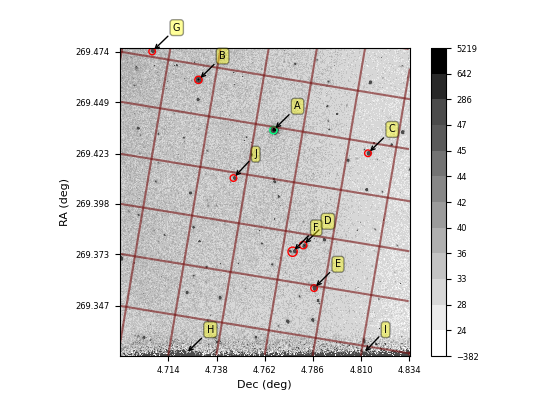
\includegraphics[scale=1]{images/initgexample.png}
\end{center}
\caption{This is an observation of {\bstar} taken with the {\gfilter} on
17 September 2018 at 02:58:52 UTC after processing using the master bias and
flat files for September 2018. The brightest object, marked \textbf{A} and marked in
green is \bstar, whilst the next 9 brightest objects are marked in yellow and
\textbf{B}, \textbf{C}, etc. in decreasing order of brightness.}
\protect\label{fig:initgexample}
\end{figure}

\begin{figure}[!htbp]
\begin{center}
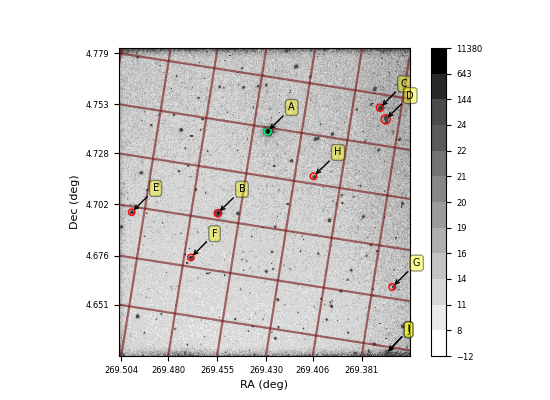
\includegraphics[scale=1]{images/initgexample20.png}
\end{center}
\caption{This is an observation of {\bstar} taken with the {\gfilter} on
7 March 2020 at 09:07:23 UTC after processing using the master bias and
flat files for March 2020. The brightest object, marked \textbf{A} and marked in
green is \bstar, whilst the next 9 brightest objects are marked in yellow and
\textbf{B}, \textbf{C}, etc. in decreasing order of brightness. It may be
noted that some of the objects, at this stage, prior to more detailed analysis
of the other objects, are not marked consistently with those in Fig. \ref{fig:initgexample}.}
\protect\label{fig:initgexample20}
\end{figure}

In nearly every case there are 4 images taken, one with each of the 4 visible
light filters (in addition to the simultaneous REMIR observations) and in Fig.
\ref{fig:initgexample} is illustrated a set of observations of {\prox} taken on
the same date, 17 September 2018, as the observation of {\bstar} in Fig.
\ref{fig:initgexample}. For comparison, in Fig. \ref{fig:init4example20} is
shown a set of observations taken on 9 March 2020.

\begin{figure}[!htbp]
\begin{center}
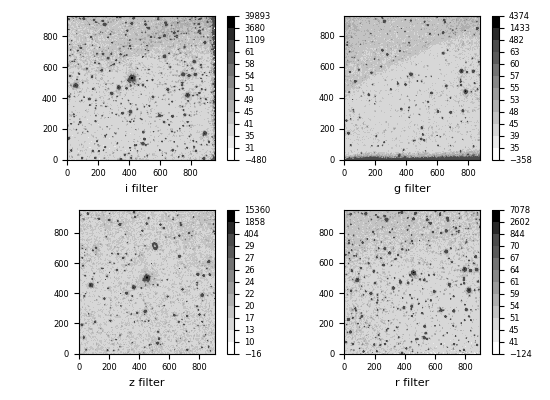
\includegraphics[scale=1]{images/init4example.png}
\end{center}
\caption{This is all 4 observations of {\prox} taken with the visible light
filters on 17 September 2018 at 02:12:40 UTC after processing using
appropriate master bias and flat files for September 2018. They are arranged in
the order and orientation in which they are taken from the CCD. The
divisions on each image are pixel numbers.}
\protect\label{fig:init4example}
\end{figure}

\begin{figure}[!htbp]
\begin{center}
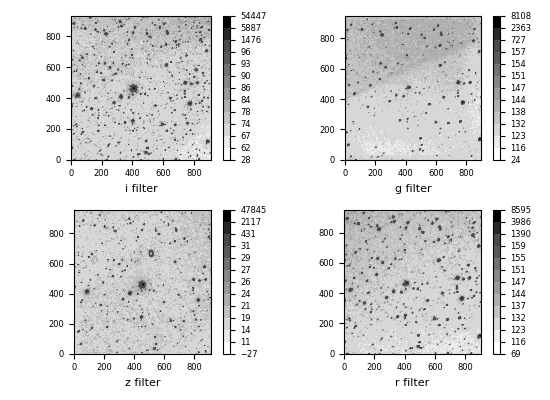
\includegraphics[scale=1]{images/init4example20.png}
\end{center}
\caption{This is all 4 observations of {\prox} taken with the visible light
filters on 9 March 2020 at 08:56:14 UTC after processing using
appropriate master bias and flat files for March 2020. They are arranged in
the order and orientation in which they are taken from the CCD. The
divisions on each image are pixel numbers.}
\protect\label{fig:init4example20}
\end{figure}

\clearpage

\subsection{Caveats and matters to be addressed in analysing data}
\protect\label{section:mattersaddressed}

The following issues were apparent in the analysis of the data.

\begin{enumerate}
  \item There is no clear uncertainty measure in the master flat and bias files.
  \item The master flat files do not appear to be adequate, with some shading in
  	the images. This is particularly of concern with the {\gfilter}
  	towards the bottom part, although this is towards the centre of the CCD, as
  	shown in Fig. \ref{fig:showusedccd}.
  \item Some of the pixel values become negative after subtraction of the master
  	bias files.
  \item There is a ring-shaped artefact above and slightly to the right of the
  	brightest objects in the images for the {\zfilter}, invariably for
	the target, but to a greater or lesser degree for the other objects. Often the
	artefact lands entirely on another object, compromising the usability of the
	frame.
\end{enumerate}

As a result, it proved advisable to avoid the {\zfilter} as it would not
be practical to try to compensate for the artefacts given the likely poor return
if this were done. The target {\rdwarf} objects are invariably very much
brighter than any of the possible reference objects for this (and also for the
\ifilter) and any extensive effort to eliminate the artefacts would not appear
worthwhile.
